\chapter{Introducing}

Firstly we will start by the introduction to the main characters -- intersection defined graph classes; characterization of chordal graphs.

\section{Intersection defined graph classes}

\begin{defn}
	The intersection graph of a set family $\mathcal{A}$ is the graph
	
	$$
	IG(\mathcal{A}) = (\mathcal{A}, \{ab : a \neq b, a \cap b \neq \emptyset, a, b \in \mathcal{A}\}).
	$$
\end{defn}

\begin{defn}
	Let $\mathcal{M}$ be a family of sets. We say that a graph $G$ is an intersection graph of (members of) $\mathcal{M}$ if $G$ is isomorphic to the graph $IG(\mathcal{A})$ for some family $\mathcal{A}$ whose all elements belong to $\mathcal{M}$. We write
	
	$$
	\mathcal{IG}(\mathcal{M}) = \{\mathcal{IG}(\mathcal{A}) : \mathcal{A} \subseteq \mathcal{M}\}.
	$$
\end{defn}

\begin{observ}
	For every graph $G$ and every set family $\mathcal{M}, G \in \mathcal{IG}(\mathcal{M})$ if and only if there is a mapping $f : V (G) \to \mathcal{M}$ such that $uv \in E(G)$ iff $f(u) \cap f(v) \neq \emptyset$ holds true for all pairs of distinct vertices $u, v$ of $G$.
\end{observ}

\begin{observ}
	For every family $\mathcal{M}$ (containing at least one nonempty set), it holds that $\mathcal{IG}(\mathcal{M}$ contains all complete graphs and is hereditary (i.e., every induced subgraph of every graph from $\mathcal{IG}(\mathcal{M})$ also	belongs to $\mathcal{IG}(\mathcal{M})$).
\end{observ}

\subsection{Examples}

In many cases, the members of $\mathcal{M}$ are defined by their geometric shape. And in most of these cases, the members of $\mathcal{M}$ are arc-connected sets in the plane.

\begin{itemize}
	\item \textbf{Interval graphs} $\text{INT} = \mathcal{IG}(\{\text{intervals on a line}\})$
	\item \textbf{Circle graphs} $\text{CIR} = \mathcal{IG}(\{\text{chords of a circle}\})$
	\item \textbf{Circular arc graphs} $\text{CA} = \mathcal{IG}(\{\text{arcs on a circle}\})$
	\item \textbf{Permutation graphs} $\text{PER} = \mathcal{IG}(\{\text{segments connecting two parallel lines}\})$
	\item \textbf{Function graphs} $\text{FUN} = \mathcal{IG}(\{\text{curves connecting two parallel lines}\})$
	\item \textbf{Polygon circle graphs} $\text{PC} = \mathcal{IG}(\{\text{polygons inscribed in a circle}\})$
	\item \textbf{Segment graphs} $\text{SEG} = \mathcal{IG}(\{\text{straight-line segments in the plane}\})$
	\item \textbf{Convex graphs} $\text{CONV} = \mathcal{IG}(\{\text{convex sets in the plane}\})$
	\item \textbf{String graphs} $\text{STRING} = \mathcal{IG}(\{\text{curves in the plane}\})$
\end{itemize}

\begin{figure}[!ht]\centering
	\begin{subfigure}{0.45\textwidth}\centering
		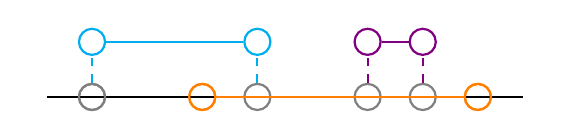
\begin{tikzpicture}[node distance={7mm}, thick, main/.style = {draw, circle}]
			\node (L) {};
			\node[main, color=gray] (1) [right of=L] {};
			\node[main, color=cyan] (11) [above of=1] {};
			\node (2) [right of=1] {};
			\node[main, color=orange] (3) [right of=2] {};
			\node[main, color=gray] (4) [right of=3] {};
			\node[main, color=cyan] (14) [above of=4] {};
			\node (5) [right of=4] {};
			\node[main, color=gray] (6) [right of=5] {};
			\node[main, color=violet] (16) [above of=6] {};
			\node[main, color=gray] (7) [right of=6] {};
			\node[main, color=violet] (17) [above of=7] {};
			\node[main, color=orange] (8) [right of=7] {};
			\node (R) [right of=8] {};
			\draw[main] (L) edge (R);
			\node[main, color=orange] (3) [right of=2] {};
			\node[main, color=orange] (8) [right of=7] {};
			\draw[color=cyan] (11) edge (14);
			\draw[color=cyan, dashed] (1) edge (11);
			\draw[color=cyan, dashed] (4) edge (14);
			\draw[color=orange] (3) edge (8);
			\draw[color=violet] (16) edge (17);
			\draw[color=violet, dashed] (6) edge (16);
			\draw[color=violet, dashed] (7) edge (17);
			\node[main, color=gray] (1) [right of=L] {};
		\end{tikzpicture}
		\caption{Drawn intervals.}
	\end{subfigure}
	\begin{subfigure}{0.45\textwidth}\centering
		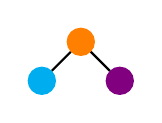
\begin{tikzpicture}[node distance={7mm}, thick, main/.style = {draw, circle, fill}]
			\node[main, color=cyan] (C) {};
			\node[main, color=orange] (O) [above right of=C] {};
			\node[main, color=violet] (V) [below right of=O] {};
			\draw (O) edge (V);
			\draw (C) edge (O);
		\end{tikzpicture}
		\caption{Corresponding graph.}
	\end{subfigure}
	\caption{Example of a graph from INT class.}
\end{figure}

\begin{figure}[!ht]\centering
	\begin{subfigure}{0.45\textwidth}\centering
		\begin{tikzpicture}[node distance={9mm}, thick, main/.style = {draw, circle}]
			\node[main, color=cyan] (L1) {};
			\node[main, color=orange] (L2) [below of=L1] {};
			\node[main, color=lime] (L3) [below of=L2] {};
			\node[main, color=blue] (L4) [below of=L3] {};
			\node[main, color=red] (L5) [below of=L4] {};
			\node[main, color=violet] (L6) [below of=L5] {};
			\node[main, color=lime] (R1) [right=2cm of L1] {};
			\node[main, color=cyan] (R2) [below of=R1] {};
			\node[main, color=violet] (R3) [below of=R2] {};
			\node[main, color=blue] (R4) [below of=R3] {};
			\node[main, color=orange] (R5) [below of=R4] {};
			\node[main, color=red] (R6) [below of=R5] {};			
			\draw[color=gray] (L1) edge (L6);
			\draw[color=gray] (R1) edge (R6);
			\draw[color=cyan] (L1) edge (R2);
			\draw[color=orange] (L2) edge (R5);
			\draw[color=lime] (L3) edge (R1);
			\draw[color=blue] (L4) edge (R4);
			\draw[color=red] (L5) edge (R6);
			\draw[color=violet] (L6) edge (R3);
		\end{tikzpicture}
		\caption{Drawn permutations.}
	\end{subfigure}
	\begin{subfigure}{0.45\textwidth}\centering
		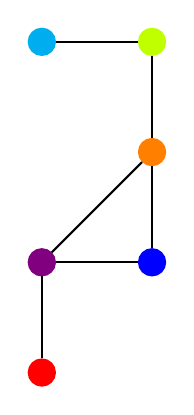
\begin{tikzpicture}[node distance={14mm}, thick, main/.style = {draw, circle, fill}]
			\node[main, color=cyan] (1) {};
			\node[main, color=lime] (2) [right of=1] {};
			\node[main, color=orange] (3) [below of=2] {};
			\node[main, color=blue] (4) [below of=3] {};
			\node[main, color=violet] (5) [left of=4] {};
			\node[main, color=red] (6) [below of=5] {};

			\draw (1) edge (2);
			\draw (2) edge (3);
			\draw (3) edge (4);
			\draw (3) edge (5);
			\draw (4) edge (5);
			\draw (5) edge (6);
		\end{tikzpicture}
		\caption{Corresponding graph.}
	\end{subfigure}
	\caption{Example of a graph from PER class.}
\end{figure}

\section{Chordal graphs}

\begin{defn}
	A graph is \textbf{chordal} if it does not contain any cycle of length greater than three as an induced subgraph.
\end{defn}

\begin{defn}
	A vertex $u$ of a graph $G$ is \textbf{simplicial} if $G[N_G(u)]$ is a clique.
\end{defn}

\begin{defn}[PES]
	A \textbf{perfect elimination scheme} for a graph $G$ is a linear ordering $u_1, u_2, \dots, u_n$ of its vertices such that for every $i, u_i$ is simplicial in the induced subgraph $G[\{u_1, u_2, \dots, u_i\}]$.
\end{defn}

\begin{lemma}
	Every minimal vertex cut in a chordal graph induces a clique.
\end{lemma}

\begin{proof}
	Let $A \subset V(G)$ be a minimal vertex cut, and suppose $u, v$ be two vertices of $A$. These vertices	are connected by a path in each component of $G \setminus A$. If $u$ and $v$ were not adjacent, a pair of shortest such paths would give rise to an induced cycle of length greater than 3 in $G$.
\end{proof}

\begin{lemma}
	Every chordal graph, which is not a complete graph, contains two nonadjacent simplicial vertices.
\end{lemma}

\begin{proof}
	By induction. If $G$ is a complete graph, the claim of the lemma is fulfilled. If $G$ is not complete, it has a vertex cut, say $A$. Let $B$ be a connected component of $G \setminus A$, and set $G_1 = G[B \cup A]$ and $G_2 = G \setminus B$. By induction hypothesis, each of $G_1, G_2$ is either complete or has two nonadjacent simplicial vertices. Thus each of them has a simplicial vertex which does not belong to $A$. Each of	these is then also simplicial in entire $G$, and they are clearly nonadjacent.
\end{proof}

\begin{cor}
	Every nonempty chordal graph contains a simplicial vertex.
\end{cor}

\begin{defn}[Clique-tree decomposition]
	A \textbf{clique-tree decomposition} of a graph $G$ is a tree $T = (\mathcal{Q}, F)$, with $\mathcal{Q}$ being the set of all maximal cliques of $G$, such that for every vertex $u \in V(G)$, the subgraph $T[\{Q : u \in Q \in \mathcal{Q}\}]$ is connected.
\end{defn}

\textbf{Warning!! The vertex set of a clique-tree decomposition of a graph G is uniquely defined, but not necessarily the edge set!!}

\begin{thm}
	For any graph $G$, the following statements are equivalent:
	
	\begin{enumerate}
		\item $G$ is chordal,
		\item $G$ allows a PES.
		\item $G$ has a clique-tree decomposition, and
		\item $G$ is an intersection graph of subtrees of a tree.
	\end{enumerate}
\end{thm}

\begin{proof}
	"$1. \Rightarrow 2.$" By induction on the number of vertices, using Lemma 2.
	
	"$2. \Rightarrow 3.$" By induction on the number of vertices again. Suppose $G' = G \setminus v_n$ has a clique-tree	$T = (\mathcal{Q}' , F')$. If $Q' = N_G (v_n) \in \mathcal{Q}'$ , then $Q = N_G [v_n]$ is a maximal clique in $G, \mathcal{Q} = (\mathcal{Q}' \setminus \{Q'\}) \cup \{Q\}$ and $T = (\mathcal{Q}, F)$ is a clique-tree for $G$, where $F = (F' \setminus \{Q' P : P \in \mathcal{Q}'\}) \cup \{QP : Q'P \in F'\}$. If, on the other hand, $Q' = N_G(v_n) \notin \mathcal{Q}'$ , then $\mathcal{Q} = \mathcal{Q}' \cup N_G [v_n]$ and $(\mathcal{Q}, F' \cup N_G [v_n]P)$ is a clique-tree for $G$ for any $P \in \mathcal{Q}'$ such that $N_G (v_n) \subset P$.
	
	"$3. \Rightarrow 4.$" Given a clique-tree decomposition $T = (\mathcal{Q}, F)$, define $T_u = T [\{Q : u \in Q \in \mathcal{Q}\}]$ for $u \in V(G)$. Clearly $V(T_u) \cap V(T_v) \neq \emptyset$ iff $u$ and $v$ belong to the same maximal clique of $G$, which happens if and only if $u$ and $v$ are adjacent in $G$.
	
	"$4. \Rightarrow 1.$" Let $G$ be the intersection graph of a collection $\{T_u\}_{u \in V(G)}$ of subtrees of a tree $T$. Suppose $v_1, v_2, \dots, v_k$ be an induced cycle in $G$, with $k > 3$. Then the subtrees $T_{v_1}$ and $T_{v_3}$ are vertex disjoint, and hence there is an edge $e \in E(T)$ which lies on every path connecting $T_{v_1}$ and $T_{v_3}$ in $T$ . This edge separates $T$ into $T_1$ and $T_2$ such that $T_{v_1}$ and $T_{v_3}$ belong to different components of $T \setminus e$, say, $T_{v_1} \subseteq T_1$ and $T_{v_3} \subseteq T_2$. One can show by induction on $i$ that for every $i \geq 3$, $T_{v_i} \subseteq T_2$. But then $T_{v_k}$ and $T_{v_1}$ must be disjoint, contradicting the assumption that $v_1 v_k \in E(G)$.
\end{proof}

\begin{cor}
	Chordal graphs are perfect (i.e., $\chi(H) = \omega(H)$ for every induced subgraph $H$ of $G$).
\end{cor}

\begin{proof}
	Consider a PES $u_1, u_2, \dots, u_n$ for $G$ and color the vertices from $u_1$ to $u_n$ by the First Fit Method (we try to use minimal color if we cannot use any of them, create a new color).
\end{proof}